\documentclass{article}
\usepackage[utf8]{inputenc}
\usepackage[a4paper, total={7in, 8in}]{geometry}
\usepackage{amsmath, amssymb}
\usepackage{bm}
\usepackage{graphicx}
\usepackage{caption}

\title{Transition path sampling and the calculation of free energies: trials and tribulations}
\author{Schwartz group}
\begin{document}
\maketitle
\section*{Probability distribution functions}

The probability distribution function for a point in the phase space ($\mathbf{x} = {\mathbf{r,p}}$) is given by 
\begin{equation}
P(\mathbf{x}) = \frac{e^{-\beta E(\mathbf{x})}}{\mathcal{Z}}
\end{equation}

The best estimate of the probability distribution from an ensemble of trajectories can be 
obtained by calculating the frequency of observing a 
The free energy for a given window with order parameter $\lambda_i$ can be obtained as 
\begin{equation}
F(\lambda_i) = -k_{B}T[ln(P(\lambda_i))] + C_i
\end{equation}
where $P(\lambda_i)$ is the probability distribution of the order parameter and $C_i$ is an 
undetermined constant which needs to be fixed to make the free energy curve continuous.  

\begin{figure}[ht]
  \centering
  \begin{minipage}[b]{0.45\linewidth}
    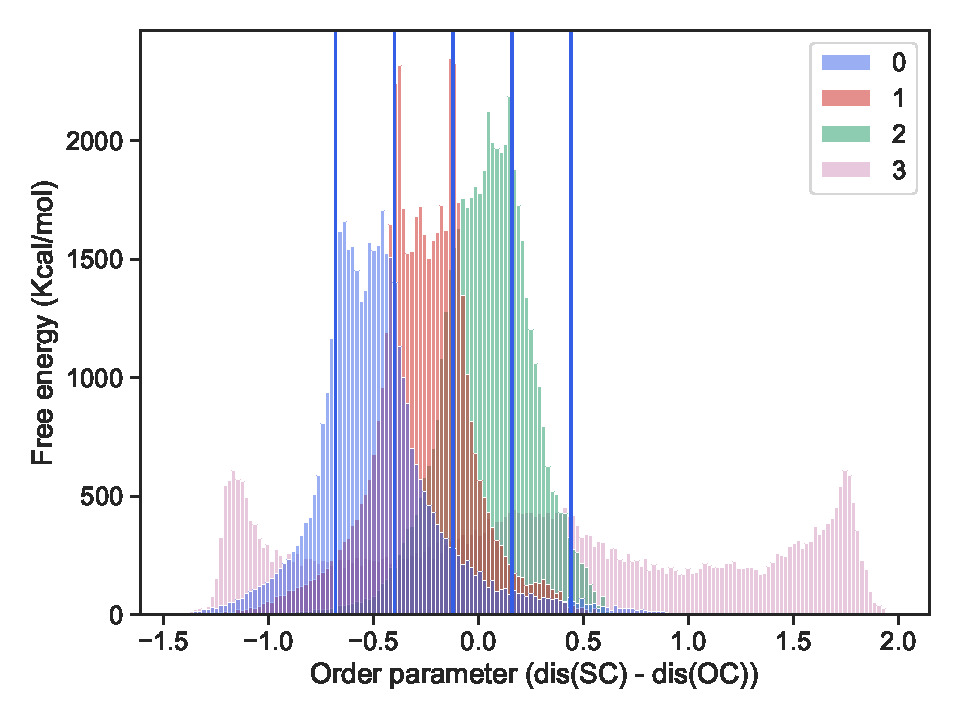
\includegraphics[scale=0.55]{figures/dist.pdf}
    \caption{Distribution of the order parameter}
    \label{fig:minipage1}
  \end{minipage}
  \quad
  \begin{minipage}[b]{0.45\linewidth}
    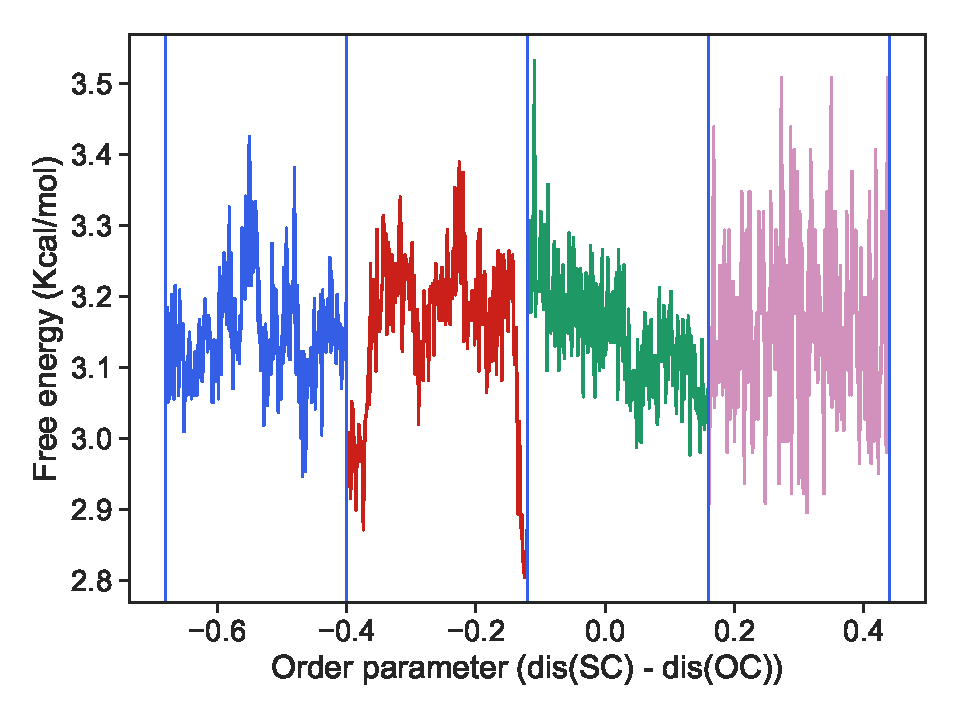
\includegraphics[scale=0.55]{figures/fenergy.pdf}
    \caption{Free energy using Boltzmann inversion}
    \label{fig:minipage2}
  \end{minipage}
\end{figure}

Figure 2 was obtained with 200 bins within each sampled window.
\end{document}
